%  Long-Short Term Memory based
% Definition of the LSTM
%
\subsubsection{Long-Short Term Memory (LSTM)-Based Models} \label{subsub:lstm}
The most commonly used time-series machine learning model is the long short-term memory cell~\cite{LSTM_Hochreiter1997}.
As in GRU, LSTM models preserve long-term dependencies in the extended data sequences.
In its ten years of existence, it has become the most widely used type of RNN in those applications.
\ifthenelse{\boolean{thesis}}{\mbox{Figure~\ref{subfig:NN-LongTerm}} summarises the internal cell logic.}
{\mbox{Figure~\ref{fig:LSTM-cell}} summarises the internal cell logic.}
%Currently, the most common usage of the Time-series Machine Learning model is the prediction of stock prices, weather prognostic or any other time-dependent data.
%However, vanishing gradient is the most common problem for any of those scenarios.
% Long-range data tend to fade away from the model, which impacts overall prediction.
\ifthenelse{\boolean{thesis}}{}{
\begin{figure}[H]%[htbp]
    % \centering
    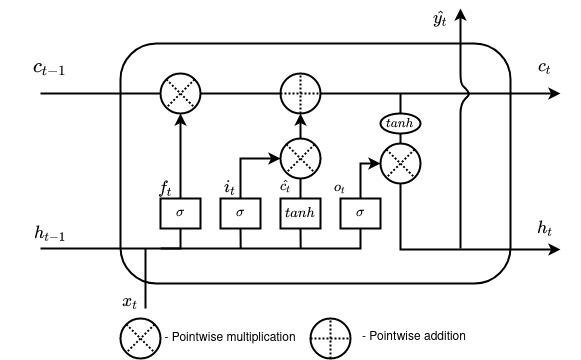
\includegraphics[width=0.80\textwidth]{II_Body/LSTM/images/LSTM.jpg}
    \caption{Structure of a long short-term memory unit cell~\cite{LSTM_Hochreiter1997}.}
    \label{fig:LSTM-cell}
\end{figure}
}
Unlike the GRU, this cell utilises three gates instead of two.
The update gate is replaced with a separate input $i_t$ and output $o_t$, as per \mbox{Equation~(\ref{eq:LSTM-gates})}.
All gates utilise the same sigmoid \mbox{Equation~(\ref{eq:sigmoid})}.
%\textcolor{red}{Those are classical LSTM approaches. Using history sizes, no Stateless methods.}
%Unlike with GRU, the update gates are renamed as an input gate $i_t$, with the same equation. Even that the forget gate $f_t$ is the same, model utilises another one, output gate $g_t$ as per Equations~\ref{eq:LSTM-gates}.
\begin{equation}
    \begin{split}
        f_t &= \sigma \left( W_f \left[ h_{t-1}, x_t \right] + b_f \right) \\
        i_t &= \sigma \left( W_i \left[ h_{t-1}, x_t \right] + b_i \right) \\
        o_t &= \sigma \left( W_o \left[ h_{t-1}, x_t \right] + b_o \right) \\
    \end{split}
    \label{eq:LSTM-gates}
\end{equation}

The main difference between the LSTM cell and the GRU lies in the cell state calculation.
Using the same $tanh$ activation function, \mbox{Equation~(\ref{eq:LSTM-output})} describes how cells are updated and propagated.
$c_t$ represents the cell state at a timestamp.
\begin{equation}
    \begin{split}
        c_t &= f_t c_{t-1}+i_t \times tanh \left( W_c \left[h_{t-1}, x_t \right] + b_c \right) \\
        h_t &= o_t*tanh \left( c_t \right)
    \end{split}
    \label{eq:LSTM-output}
\end{equation}   
% $c_t \rightarrow$ cell state (memory) at timestep $t$ \\
% $\hat{c_t} \rightarrow$ candidate for cell state \\
% $* \rightarrow$ element-wise multiplication \\
% Like the GRU cell type, the model training Library supports stateful and stateless utilisation of the LSTM model.
% It will be used as a Stateless cell for further comparison based on Chemali et al.~\cite{Chemali2017} and similar articles.

%  Attention layer
% Attention intro and explanation
% (7) \textcolor{red}{The most complicated one}. The method by WeiZhang2020. Adaptive Time-series prediction on online validation. Data were taken directly during cycling batteries.
% \textbf{I have to study this properly first. Long-Horizon, as they called it, was more useful to the State of Health. This should be the end of them.}
%  Attention Layer
% Introduction and origins of attention usage
%
\subsubsection{LSTM with Attention Layer}
The research conducted by Mamo and Wang~\cite{mamo_long_2020} was intended to determine weaknesses and improve the LSTM structure by introducing additional techniques to the default layer of the training model.
They added an attention layer~\cite{yang_hierarchical_2016} between the LSTM and fully connected layers to improve accuracy and replaced a traditional gradient optimiser with a probability-based differential evolution.
\mbox{Figure~\ref{fig:attention}} summarises the model structure, and \mbox{Equations~(\ref{eq:AttentionWithContext})} and~(\ref{eq:Addition}) define the internal logic between hidden layers and output.

% The origins of the source code
%
%bla bla bla... I am exosted, I hate this part; I have no idea what to write and have no desire to research more.
The implementation of the attention layer was not provided with the machine learning library.
The source code from Winata and Kampman's research~\cite{winata_attention-based_2018} was used instead.
The open-source code is publicly accessible through its Github source~\cite{winata_attention-based_2018}.
Details of the optimiser usage and replacement are presented in Section~\ref{subsec:optimisers}.
In the state-of-charge estimation, the attention layer addresses the LSTM shortcomings, such as replacing the traditional method of recursively constructing the LSTM depth, and locating it after the output of the primary layer, just before the model's dense layer output~\cite{mamo_long_2020}.
\vspace{6pt}
\begin{equation}
    \begin{split}
        u_t &= tanh \left(W h_{t} + b \right) \\
        \alpha_t &= \frac{exp(u^T u)}{\sum_t(exp(u_t^T u))} \\
        v_t &= \alpha_t*h_t
    \end{split}
    \label{eq:AttentionWithContext}
\end{equation}
\begin{equation}
    \begin{split}
        v = \sum_t(\alpha_t * h_t)
    \end{split}
    \label{eq:Addition}
\end{equation}

\vspace{-6pt}
\begin{figure}[H]
    % \centering
    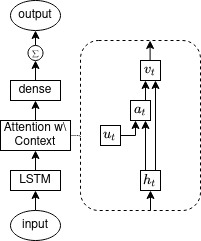
\includegraphics[width=0.55\linewidth]{II_Body/LSTM/images/AttenrionDrawing.jpg}
    \caption{Attention-based architecture.}
    \label{fig:attention}
\end{figure}
%
% \subsection{Implementation}
%     Following table highlights parameters which provided the best results for their experiments.
%     \textbf{Table of the parameters.}
%     The network will be the one discussed above.
%     Model itself will be multi-feature based with follwoing parameters: Voltage \textit{V(t)}, Current \textit{A(t)} and Temperature \textit{C(t)}, where \textit{t} represents a time-stamp. Each feature will contain an equal amount of sample and feed in the input column vector. As a result, a single input will have the following form: \\
%     % [V(0)], [I(0)], [T(0)] \\
%     % [V(1)], [I(1)], [T(1)] \\
%     % [V(n)], [I(n)], [T(n)] \\
%     where \textit{n} is the history size.
%     The output vector will be a State of Charge \textit{SoC(\%)} percentage up to 2 decimal places, within range 0 to 1 and time stamp \textit{n}: \\
%     % [SoC(n)] \\
%     As a result, the shape of input and output data will be: X(0)=(n,3) and Y(0)=(1)
%     The entire dataset will use a single-step windowing technique with no batches to save memory and utilise \textbf{stateless}* \footnote{Need to discuss this with Holmes.} model. \\
%     The Generated dataset of sample size \textit{k}, will consist of two Tensor input/output Vectors of the following shape: \\
%     X = (k-n,n,3), Y = (k-n,1).
%     The variable type for computation was selected to be float32.
%     To keep the Denerated dataset simple, no batching approach spared from dealing with 4-dimensional input vectors.
% \subsection{Prediction results}
%     Implementation of the model based on Chemali2017—application for our section and results. Refer to methodology from time to time.